\chapter{Deformed Nuclei}

\section{Nuclear deformation}

Most of the nuclei across the nuclide chart are spherical or symmetric in their ground state. Moreover, for the axially symmetric nuclei (i.e, either \emph{oblate} or \emph{prolate}), there is a prolate over oblate dominance.
% \begin{figure}[ht]
%     \centering
%     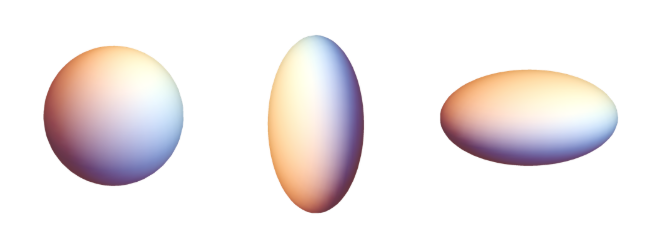
\includegraphics[scale=0.3]{Chapters/Figures/nuclear_shapes.png}
%     \caption{Nuclear Shapes.}
%     \label{nuclear_shapes}
% \end{figure}

The spherical shell model only describes nuclei near the closed shells. On the other side, for the nuclei that lie far from closed shells, a deformed potential must be employed. 
\par In the case of even-even nuclei, unique band structures resulting from the vibrations and rotations of the nuclear surface (as proposed by Bohr and Mottelson \cite{bohr1998nuclear} in the \emph{Geometric Collective Model} - GCM) appear in the energy range 0-2 MeV.

Within the GCM, the nucleus is described as a classical charged liquid drop. For the low-lying energy spectrum, usually, the compression of nuclear matter and the nuclear skin thickness are neglected. This results in the final picture of a liquid drop with a constant nuclear density and a sharp surface \cite{greiner1996nuclear}.

\subsection{Collective coordinates}

The nuclear surface can be described via an expansion of the spherical harmonic functions with some time-dependent parameters as \emph{expansion coefficients}. The expression of the nuclear shape is shown below \cite{greiner1996nuclear}:
\begin{align}
    R(\theta,\varphi,t)=R_0\left(1+\sum_{\lambda=0}^\infty\sum_{-\lambda}^\lambda\alpha_{\lambda\mu}(t)Y_\lambda^\nu(\theta,\varphi)\right)\ .
    \label{nuclear-shape}
\end{align}

In \ref{nuclear-shape}, $R$ denotes the nuclear radius as a function of the spherical coordinates $\theta,\varphi)$ expressing the direction, and the time $t$, while $R_0$ is the radius of the spherical nucleus when all the expansion coefficients vanish. It is worth mentioning that the expansion coefficients $\alpha_{\lambda\mu}$ act as \emph{collective coordinates} since the time-dependent amplitudes describe the vibrations of the nuclear surface.

\subsection{Nuclear radius under rotation}

To get a grasp at the physical meaning behind the deformation parameters that are used to describe the nuclear surface, it is instructive to see what happens when the system undergoes a rotation transformation.

The function $R(\theta,\varphi)$ describes the original (non-rotated) nuclear shape. Rotating the system will result in the change of the angular coordinates $(\theta,\varphi)$ to $(\theta',\varphi')$, which will correspond to a new function $R'(\theta',\varphi')$. Moreover, both nuclear surfaces (i.e., the non-rotated and the rotated one) must hold the equality:
\begin{align}
    R'(\theta',\varphi')=R(\theta,\varphi)
\end{align}

The rotational invariance of $R$ employs that $R'(\theta,\varphi)$ must have the same functional form, but the expansion coefficients $\alpha_{\lambda\mu}$ must be rotated, meaning:
\begin{align}
    \sum_{\lambda\mu}\alpha_{\lambda\mu}'Y'_{\lambda\mu}(
        \theta,\varphi)=\sum_{\lambda\mu}\alpha_{\lambda\mu}Y_{\lambda\mu}(
            \theta,\varphi)\ . \label{nuclear_surface_equality}
\end{align}

Note that in Eq. \ref{nuclear_surface_equality}, the spherical harmonics $Y'_{\lambda\mu}$ are obtained via the usual rotation matrices. Finally, the invariance of Eq. \ref{nuclear-shape} is achieved if the set of parameters $\alpha_{\lambda\mu}$ transform similarly to a \emph{spherical tensor with angular momentum} $\lambda$ \cite{ring2004nuclear}, that is:
\begin{align}
    \alpha_{\lambda\mu}'=\sum_{\mu'}\mathcal{D}^{(\lambda)}_{\mu\mu'}\alpha_{\lambda\mu'}\ .
\end{align}

Besides the spherical tensor character, the collective coordinates also have the following properties (emerging from Eq. \ref{nuclear-shape}):
\begin{itemize}
    \item Complex Conjugation.
    \begin{align}
        Y^*_{\lambda\mu}(\theta,\varphi)&=(-1)^{\mu}Y_{\lambda-\mu}(\theta,\varphi), \\
        \alpha^*_{\lambda\mu}&=(-1)^\mu\alpha_{\lambda-\mu}\ .
    \end{align}
    \item Parity - the coordinates $\alpha_{\lambda\mu}$ must undergo the same change of sign under a parity transformation as the spherical harmonics, in order to keep the invariance of the nuclear surface.
    \begin{align}
        (r,\theta,\varphi) &\xrightarrow[P]{}     (r,\pi-\theta,\pi+\varphi)\ \nonumber, \\
        Y_{\lambda\mu}(\theta,\varphi) &\xrightarrow[P]{} Y_{\lambda\mu}(\pi-\theta,\pi+\varphi)=(-1)^\lambda Y_{\lambda\mu}(\theta,\varphi)\ .\nonumber
    \end{align}
    Therefore, the parity of the expansion coefficients are:
    \begin{align}
        \pi(\alpha_{\lambda\mu})=(-1)^\lambda\ .
    \end{align}
\end{itemize}

\subsection{Multipole deformations}

In the expansion of the nuclear surface defined by Eq. 
\ref{nuclear-shape}, the different values for $\lambda$ will determine different effects regarding the physical aspects of the nucleus. As such, the first values of $\lambda$ will be examined in terms of the physical meaning.

\begin{description}
    \item[Monopole mode] This corresponds to the first value of $\lambda=0$. This is the simplest mode of \emph{deformation} of a nuclear surface. Within this approximation, the spherical harmonic $Y_0^0$ is constant, which would imply that any non-vanishing values for $\alpha_{00}$ will correspond to the change in radius of the nucleus. This kind of excitation is also called \emph{breathing mode} of the nucleus \cite{greiner1996nuclear,bohr1998nuclear}. The energy required for this kind of excitation mode is very large, since it implies a compression of the nuclear matter. As a result, this mode is irrelevant in the low-lying excited spectra of atomic nuclei.
    \item[Dipole mode] Corresponds to $\lambda=1$. In reality, this type of mode does not manifest itself as a deformation of the nucleus, but rather as a shift of the nuclear center of mass. In the lowest order $\lambda=1$, the shift is in fact a translation of the entire nucleus, and it does not represent an actual nuclear excitation.
    \item[Quadrupole mode] Excited modes that correspond to $\lambda=2$. These are the most important collective excitations that take place inside the nucleus. The loss of axial symmetry, triaxial deformations, and other shape-specific transitions that happen within the nucleus are mostly described (and very accurately) via the quadrupole effects.
    \item[Octupole mode] This corresponds to the next increasing value of $\lambda=3$, representing the main asymmetric excitations of a nucleus with states of negative-parity. The specific shape of a nuclear system governed by octuple deformations is similar to that of a pear.
    \item[Hexadecupole deformations] Excitations which correspond to $\lambda=4$. Within the nuclear theory, this is considered the highest angular momentum which can still provide relevant information for the nuclear phenomena that are studied. Currently, there is no clear evidence for pure excitations with hexadecupole nature, however, these excitations seem to have a major role in the admixture to quadrupole excitations for the ground-state shape of heavy nuclei \cite{greiner1996nuclear}.
\end{description}
The multipole deformations for the cases $\lambda=1,2,3$ and $\lambda=4$ discussed above are pictorially shown in Fig. \ref{multipole-deformations}.
Excitations with higher angular momentum than the mentioned ones have practically no application within the study of atomic nuclei. Moreover, one can also see that there is an intrinsic limitation on the maximal value of $\lambda$, which dictates the smallness of the individual bumps of the surface (see Fig. \ref{multipole-deformations}). These bumps are described by the spherical harmonics $Y_\lambda^\mu$, and they decrease in size with increasing values of $\lambda$, but with the physical limitation given by the size of the nucleon diameter.

\begin{figure}
    \centering
    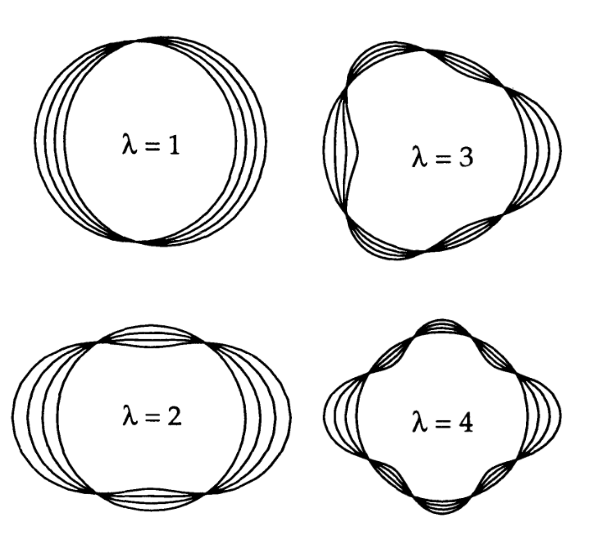
\includegraphics[scale=0.3]{Chapters/Figures/nuclearDeformation.png}
    \caption{Graphical representation for the first few modes of excitations of the nuclear surface. The figure is taken from Ref. \cite{greiner1996nuclear}.}
    \label{multipole-deformations}
\end{figure}

\subsection{Quadrupole Deformation}

One of the most important excitation modes (vibrational degrees of freedom) is the quadrupole deformation, corresponding to $\lambda=2$. In the case of pure quadrupole deformation, the nuclear surface will be given by the following expression:
\begin{align}
    R(\theta,\varphi)=R\left(1+\sum_\mu\alpha_{2\mu}Y_2^\mu(\theta,\varphi\right)\ . \label{quadrupole-surface}
\end{align}

An important remark is that the expansion coefficients (i.e., $\alpha_{2,\mu}$ parameters) from Eq. \ref{quadrupole-surface} are not all independent. The parameters $\alpha_{2,\mu}$ follow the same complex conjugation relation as the spherical harmonics $Y_2^0$ do, keeping thus $\alpha_{20}$ real. The coefficient $\alpha_{00}$ is the \emph{volume-conserving} term \cite{greiner1996nuclear,ring2004nuclear}. These two aspects imply that there are only five real and independent degrees of freedom for the nuclear deformation: the volume term $\alpha_{00}$, the real parts of $\alpha_{21},\alpha_{22}$, and the imaginary parts of $\alpha_{21},\alpha_{22}$, respectively.

A complete set of calculations for the nuclear radius $R(\theta,varphi)$, expressed in terms of cartesian coordinates (done by re-writing the spherical harmonics in terms of cartesian components of the unit vector pointing in a particular direction given by $(\theta,\varphi)$) is done by in \cite{greiner1996nuclear}. Therein, it was concluded that the five parameters describing the nuclear shape for the quadrupole excitations can be interpreted as such:
\begin{itemize}
    \item $\alpha_{20}$ parameter describes the stretching of the $z$ axis with respect to the $y$ and $x$ axes.
    \item $\alpha_{2-2}$ and $\alpha_{22}$ parameters give the relative length of the $x$ axis compared to the $y$ axis. Moreover, it also gives the oblique deformation in the $x-y$ plane.
    \item $\alpha_{2-1}$ and $\alpha_{21}$ parameters also describe an oblique deformation, but with respect to the $z$ axis.
\end{itemize}

With the set of parameters defined above, the shape and orientation of the nucleus can have arbitrary values (the coefficients $\alpha_{2\mu}$ are mixing in this way the shape and orientation), thus making the parametrization somewhat problematic.

In order to fix that, the geometry can be changed if one considers the \emph{principal axis system} (the PA reference system is a coordinate system in which the moments of inertia associated with the nucleus are diagonal). When using this reference frame, the number of parameters is still unchanged, however their physical significance becomes clearer:
\begin{itemize}
    \item $a_0$ is indicating the stretch of $z'$ axis w.r.t. the $x'$ and $y'$ axes.
    \item $a_2$ is indicating the asymmetry between the lengths of $x'$ and $y'$ axes respectively.
    \item Three \emph{Euler angles} $\mathbf{\theta}=(\theta_1,\theta_2,\theta_3)$. These angles will determine the orientation of the PA system $(x',y',z')$ with respect to the laboratory-fixed frame $(x,y,z)$.
\end{itemize}